\chapter{Transformer} \label{ch:transformer}

\myabb{Large language model}{LLM} is one of the many solutions to NLP, and NLP is a type of problem under sequential data processing. In the past few years we have seen revolutionary development in LLM, and hence it forms a dedicated part in the notebook. With the introduction of multimodal LLM, the capability of LLM expands beyond language processing towards image and even video processing. 

Modern LLM is built on top of Transformer, an AI framework proposed in the landmark paper ``Attention Is All You Need'' \cite{vaswani2017attention}. Transformer is introduced in this chapter. 

A brief review of RNN, the state-of-the-art framework priori to Transformer, is given, and its shortages are addressed. Transformer framework and its key components are introduced. Lastly, the development trend of Transformer is discussed.

\section{RNN and Its Limitations}

RNN has been introduced in earlier Chapter \ref{ch:rnn}. A brief review is given in this section, focusing on its shortages in NLP.

\subsection{A Brief Review of RNN}

Comparing with a dense ANN, RNN is more efficient in building up correlation between consecutive inputs, and hence it becomes a powerful framework when comes to sequential data processing. 

In a conventional dense ANN, the correlation cannot be captured efficiently. In contrast, a dense ANN would treat all the inputs ``equally'' in a symmetric manner. To enforce the ANN to ``address'' the correlation, it would require a lot more layers and nodes (which is often considered low-efficient), and requires more data points during the training. Other problems of conventional dense ANN include, for example, the lack of ability in handling data with arbitrary length.

CNN and RNN try to tackle the above problems by implementing a ``pre-processing'' stage, where the correlation of the spacial and sequential data is first abstracted using some mechanism, and the correlation information is sent as (additional) inputs to the followed dense ANN.

\subsection{Limitations of RNN}

``Attention'' was not a new concept invented in \cite{vaswani2017attention}. It was proposed a few years earlier than the transformer, and had been integrated into several CNN and RNN models to boost their performances to capture long-range dependencies. In these researches, attention mechanism is more often a supporting role than the main character. It is quite surprising indeed that when getting rid of CNN and RNN and purely relying on attention mechanism, everything gets better: more efficient in training and better in performance.

Does this mean that the RNN, which we had been relying on so much, is in fact the drawback to NLP? The following is the answer of ChatGPT-4 of this question.

\begin{mdframed}
	\textbf{Q: By getting rid of RNN and using attention mechanism alone, natural language processing performance gets better. Is this correct? Does this mean that RNN is a drawback to natural language processing?}
	
	A: Yes, by getting rid of RNNs and using the attention mechanism alone, the Transformer model demonstrated improved performance in natural language processing tasks. However, it's important to note that RNNs are not inherently a drawback to NLP; they were successfully used for many tasks before the advent of Transformers.
	
	RNNs, particularly LSTM (Long Short-Term Memory) and GRU (Gated Recurrent Unit) variants, were designed to handle sequences and capture dependencies in the data. They have been effective in many NLP tasks, such as language modeling, machine translation, and sentiment analysis. However, RNNs do have certain limitations, such as difficulty in capturing long-range dependencies and sequential processing, which can lead to slower training and inference times.
	
	The attention mechanism, as employed in the Transformer model, addresses some of these limitations. It enables parallel processing of input sequences, leading to faster training and inference, and effectively captures long-range dependencies without the vanishing gradient problem that can affect RNNs.
	
	While Transformers have shown superior performance in many NLP tasks, RNNs still have their place in certain scenarios, especially when working with resource-constrained environments or smaller datasets. They can be more lightweight and computationally efficient compared to large-scale Transformer models.
	
	In summary, RNNs are not a drawback to NLP per se, but their limitations have been mitigated by the introduction of the attention mechanism in Transformer models, which has led to improved performance in a wide range of NLP tasks.
	
	(April 14, 2023, ChatGPT-4)
\end{mdframed}

\section{Transformer Framework}

A summary of the concepts, components and technologies in \cite{vaswani2017attention} is given in this section.

\subsection{Tokenizer}

In most NLP solutions, human language components need to be mapped to numbers before inputting into a model. The outputs of the model must then be mapped back to human-readable components so that a human can interpret them. This is no exception for LLMs. This mapping process is known as \mync{tokenization}.

There are multiple ways to perform tokenization. Different models, and models for different languages, may apply different tokenization schemes. In this section, English is used as an example. Commonly seen tokenization methods are discussed.

\vspace{0.1in}
\noindent \textbf{Character-Based Tokenization}
\vspace{0.1in}

The most intuitive approach is character-based tokenization. For example, we can use the ASCII standard as the mapping table, where each English character, including spaces and most commonly used special characters, is mapped to an integer.

The benefits of using character-based mapping include:
\begin{itemize}
	\item Flexibility. Everything can be mapped without exception, including typos or invented words.
	\item Compact vocabulary. To cover all characters, we need only a few dozen entries in the mapping table.
\end{itemize}

The main drawback of character-based mapping is inefficiency. For instance, consider the character sequence ``t'', ``h'', and ``e''. When they appear together, they form the word ``the'' which carries a specific and frequent meaning. Ideally, such frequent patterns should be recognized as a whole. By storing this combination in the token mapping (rather than learning it from model parameters), we can improve modeling efficiency and reduce sequence length.

\vspace{0.1in}
\noindent \textbf{Word-Based Tokenization}
\vspace{0.1in}

To improve efficiency and reduce the number of input tokens, word-based tokenization was proposed. A dictionary containing around $30{,}000$ to $50{,}000$ words is often used in common applications. Any unrecognized word such as typo or extremely rare word is mapped to a special token that represents an ``unknown'' word.

The advantages of word-based mapping include:
\begin{itemize}
	\item Efficiency. Fewer tokens are needed to represent a sentence compared to character-level mapping.
	\item Better contextual grounding. Each token usually corresponds to a semantically meaningful unit.
\end{itemize}

However, word-based tokenization sacrifices flexibility. Unseen or misspelled words provide no meaningful signal other than ``unknown''. 

Additionally, word-based schemes often ignore the semantic structure within a word. For example, consider the word ``handcraft''. It is clearly composed of two recognizable words ``hand'' and ``craft''. Semantically, ``handcraft'' relates to both. Yet, in the word-based mapping, ``hand'', ``craft'' and``handcraft'' are treated as entirely unrelated tokens. In such cases, it would be more effective to break the word into meaningful segments and tokenize those instead.

\vspace{0.1in}
\noindent \textbf{Subword-Based Tokenization}
\vspace{0.1in}

Modern LLMs typically use subword-based tokenization. This approach lies between character-based and word-based methods. It tries to achieve optimum flexibility and efficiency by smartly breaking a word into semantically meaningful chunks known as ``subwords''.

An example is given in Fig. \ref{fig:tokenizer}, where a small piece of text is tokenized using a tokenizer. From the example, we can see that while basic and commonly used words such as ``I'', ``am'', ``demonstrating'', ``sentence'' remain in one token, the sophisticated words such as ``OpenAI'', ``tokenization'', ``semantically'' are broken into subwords. Notice that spaces and special characters such as period ``.'' are also considered as part of tokens, as they carry meanings.

\begin{figure}[!htb]
	\centering
	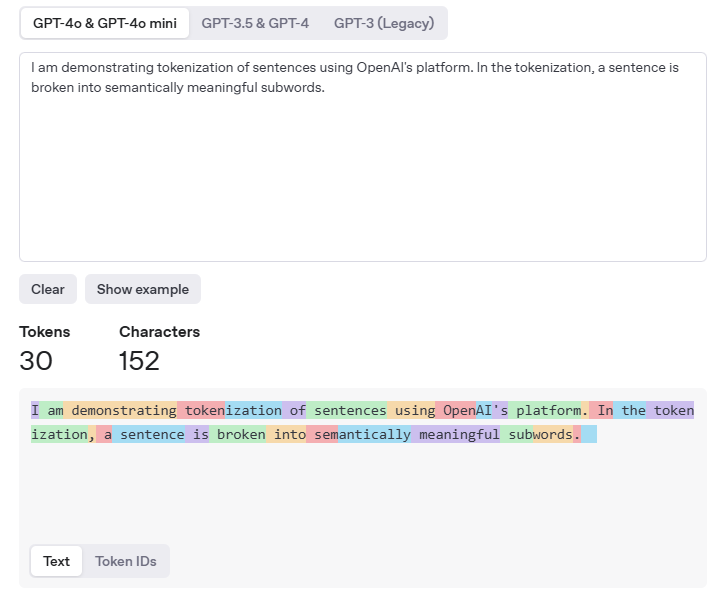
\includegraphics[width=0.75\textwidth]{./chapters/part-7/figures/tokenizer.png}
	\caption{A demonstrative example where a piece of text is tokenized using GPT-4o's tokenizer.}
	\label{fig:tokenizer}
\end{figure}

Each token is then assigned with a token ID. In the example in Fig. \ref{fig:tokenizer}, they are
\begin{lstlisting}
[40, 939, 73405, 6602, 2860, 328, 40536, 2360, 7788, 17527, 885, 6361, 13, 730, 290, 6602, 2860, 11, 261, 21872, 382, 17162, 1511, 2743, 175665, 33329, 1543, 10020, 13, 256]
\end{lstlisting}

Subword tokenization allows the model to:
\begin{itemize}
	\item Represent rare or unknown words by combining familiar parts (e.g., prefixes, stems, suffixes).
	\item Reduce the number of out-of-vocabulary tokens. Even if a new word or typo is detected in the text, it is possible that it still contains meaningful subwords.
	\item Maintain a compact vocabulary while preserving semantic structure.
\end{itemize}

Just to put things into perspective, for a typical tokenizer on English writing, $1$ token is roughly $4$ characters, or $0.75$ word, and $1000$ tokens are roughly $750$ words. Nowadays, math equations, scientific terms and codes are also used as inputs and outputs to LLMs for domain knowledge related tasks. They usually consumes more tokens than English writings.

Different LLMs may use different tokenizers. Popular subword techniques include Byte Pair Encoding, WordPiece, and Unigram tokenization. The example in Fig. \ref{fig:tokenizer} demonstrates the tokenizer of OpenAI's GPT-4o. There are many other tokenizers used by variety of models. At this point, there is not a universally best tokenizer.

The maximum number of tokens an LLM can process, both as input and output, is limited by its \mync{context window}. For example, consider a continuous dialogue with an LLM-based chatbot. Each time the user provides a new input, the entire chat history (including all of the user's previous inputs and the LLM's previous responses) is bundled together and sent as a new stateless input to the model. Based on this complete input sequence, the LLM then generates its latest response. This stateless nature means that the LLM does not ``remember'' anything beyond what is explicitly included in the current input. 

As the conversation grows longer, more and more tokens are needed to represent the chat history. For example, GPT-4o model has a context window of $128K$ tokens, roughly one-tenth the length of the complete works of Shakespeare. Once this limit is reached, older parts of the conversation must be truncated or summarized.

In some scenarios, the input cannot be easily compressed or truncated and must be passed to the LLM as a whole. For example, when an LLM is used to troubleshoot a piece of code, the entire code block, possibly including multiple files, configurations, and logs, needs to be input at once to maintain context and correctness. In such cases, the size of the context window becomes a critical constraint. If the total input exceeds the model's maximum token limit, the model will either fail to process it entirely or may be forced to omit important parts of the input, potentially leading to incorrect or incomplete responses.



\subsection{Encoder and Decoder}

TBA

\subsection{Attention Mechanism}

TBA

\subsection{Transformer-Based NLP}

\section{Transformer Development Trend}

\subsection{Transformer Variants}

\subsection{Trend}

With the sizes and capabilities of the frontier models scaling up over the past years, the models are more and more appear to be intelligent and human-like. 

A new job opportunity, ``prompt engineer'', has emerged. The workscope of a prompt engineer is to design the appropriate prompt that instructs an LLM to complete certain tasks accurately and efficiently. People starts to take advantage of LLMs in their production. 

Today, some most popular LLM applications include at least the following.
\begin{itemize}
  \item Chatbot and customer service.
  \item Copilot
  \item Agentization
\end{itemize} 